%
% $RCSfile: categorisation_versus_composition.tex,v $
%
% Copyright (C) 2002-2008. Christian Heller.
%
% Permission is granted to copy, distribute and/or modify this document
% under the terms of the GNU Free Documentation License, Version 1.1 or
% any later version published by the Free Software Foundation; with no
% Invariant Sections, with no Front-Cover Texts and with no Back-Cover
% Texts. A copy of the license is included in the section entitled
% "GNU Free Documentation License".
%
% http://www.cybop.net
% - Cybernetics Oriented Programming -
%
% http://www.resmedicinae.org
% - Information in Medicine -
%
% Version: $Revision: 1.1 $ $Date: 2008-08-19 20:41:05 $ $Author: christian $
% Authors: Christian Heller <christian.heller@tuxtax.de>
%

\subsection{Categorisation versus Composition}
\label{categorisation_versus_composition_heading}
\index{Categorisation versus Composition}
\index{Object Oriented Programming}
\index{OOP}
\index{Fragile Base Class Problem}
\index{Misuse of Inheritance}
\index{Granularity}

Since the beginnings of \emph{Object Oriented Programming} (OOP), several of
its paradigms were reflected critically and found to cause problems. One of
them is the \emph{Fragile Base Class Problem} explained in section
\ref{fragile_base_class_heading}.

\begin{figure}[ht]
    \begin{center}
        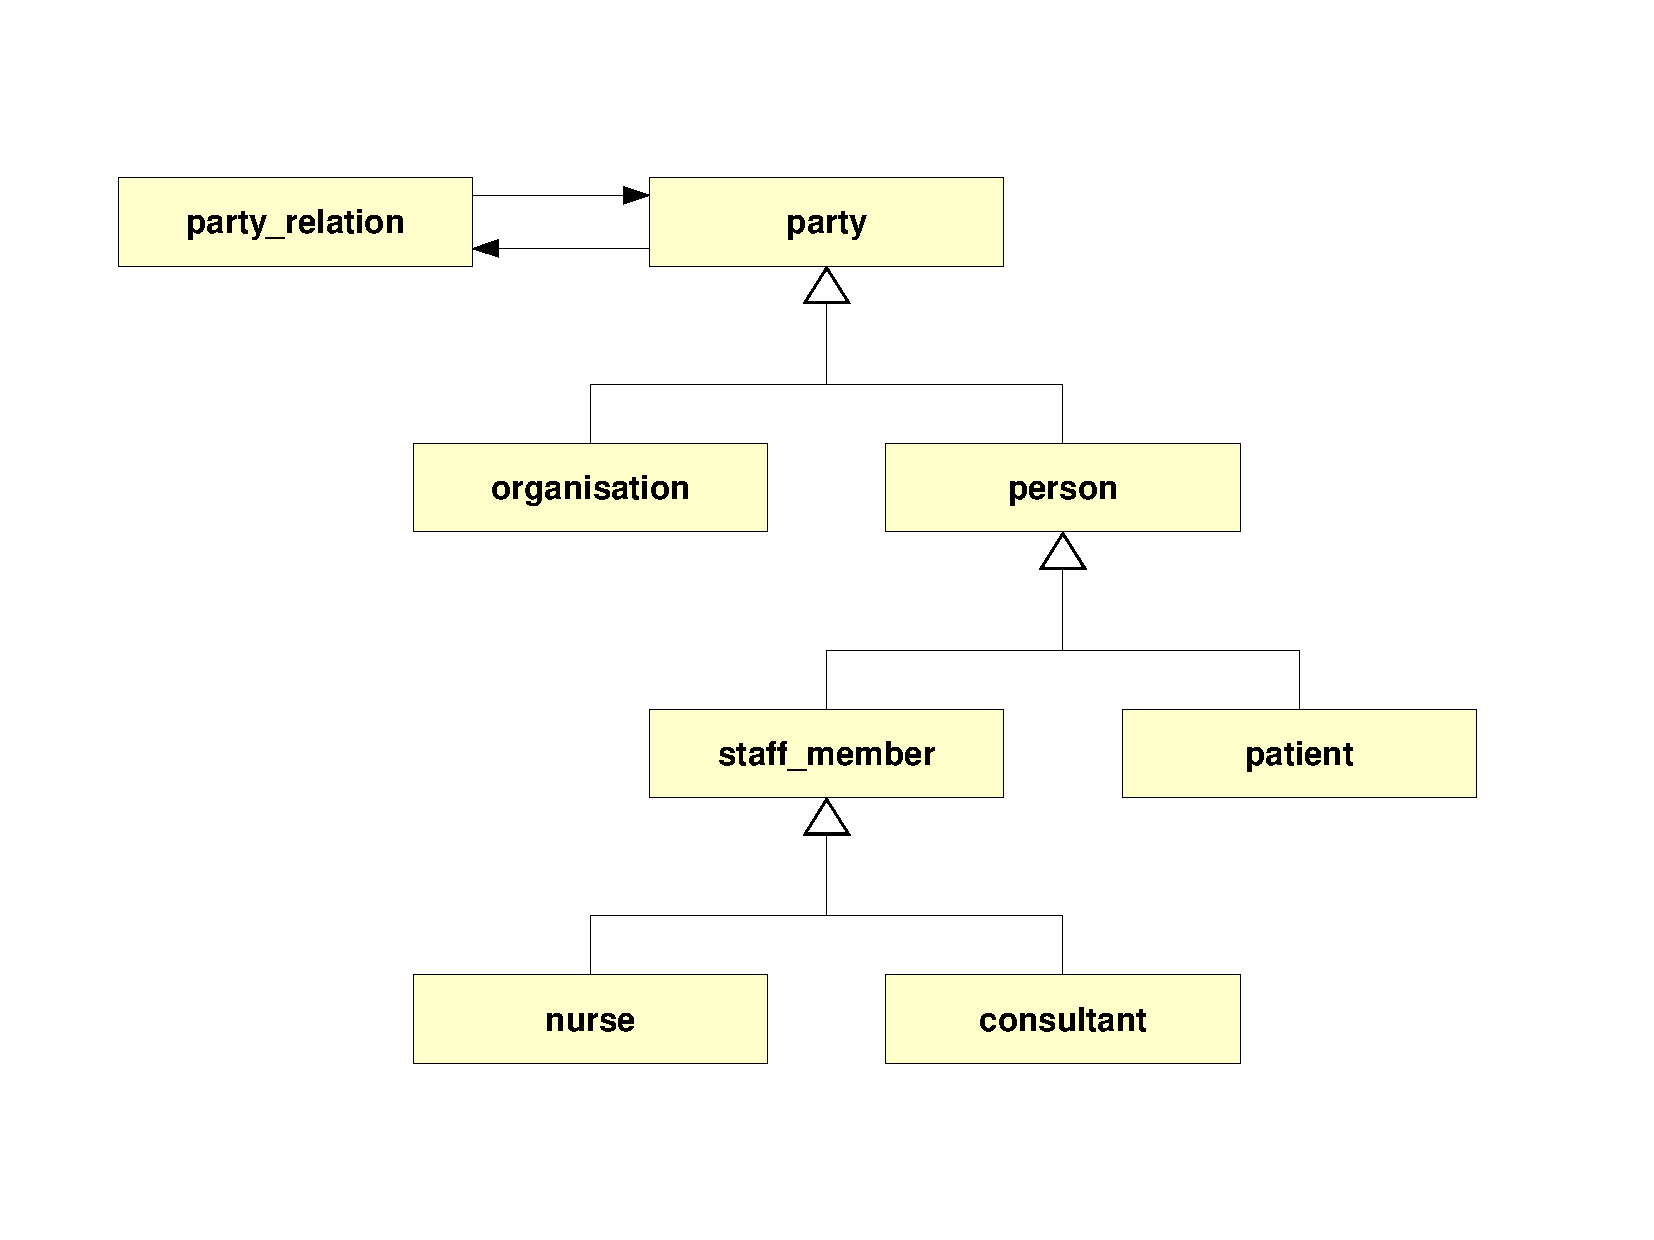
\includegraphics[scale=0.3,angle=-90]{graphic/party.pdf}
        \caption{Categorisation versus Composition of Parties \cite[p. 12]{archetypes}}
        \label{party_figure}
    \end{center}
\end{figure}

Further problems may occur through the misuse of inheritance, leading to bad
design solutions. A typical example is the modelling of demographic entities
like \emph{Patient} or \emph{Nurse} as subtypes of \emph{Person} (figure
\ref{party_figure}), whilst actually, they are \emph{Party Relationships}
\cite[p. 12]{archetypes}, \cite{fowler1997}.

As can be seen, inheritance can create more problems than are foreseeable. One
way to circumvent unwanted dependencies is to sort abstract models according to
their placement within a larger model surrounding them. Part models of a model
may be grouped by their level of \emph{Granularity}. It should never be only
\emph{Properties} leading to the creation of a super category.

A main reason for using inheritance is the reuse of functionality in form of
methods. If methods as logic models were kept externally of state models,
inheritance as way to reuse methods would not be necessary anymore (section
\ref{state_and_logic_heading}).
